\section{ADC in Study}
\label{sec:adc_in_study}

This section explains the working principle of the 12-bit asynchronous SAR ADC in study depicted in Figure \ref{fig:ADC-arch-paper}, as well analyzes the key architectural innovations implemented in this ADC. These design choices enable the ADC to achieve its remarkable $6.94 \si{\femto \joule}/conversion-step$ figure of merit while maintaining 12-bit precision at a $100 \si{\mega S \per \second}$ sampling rate.

\begin{figure}[H]
    \centering
    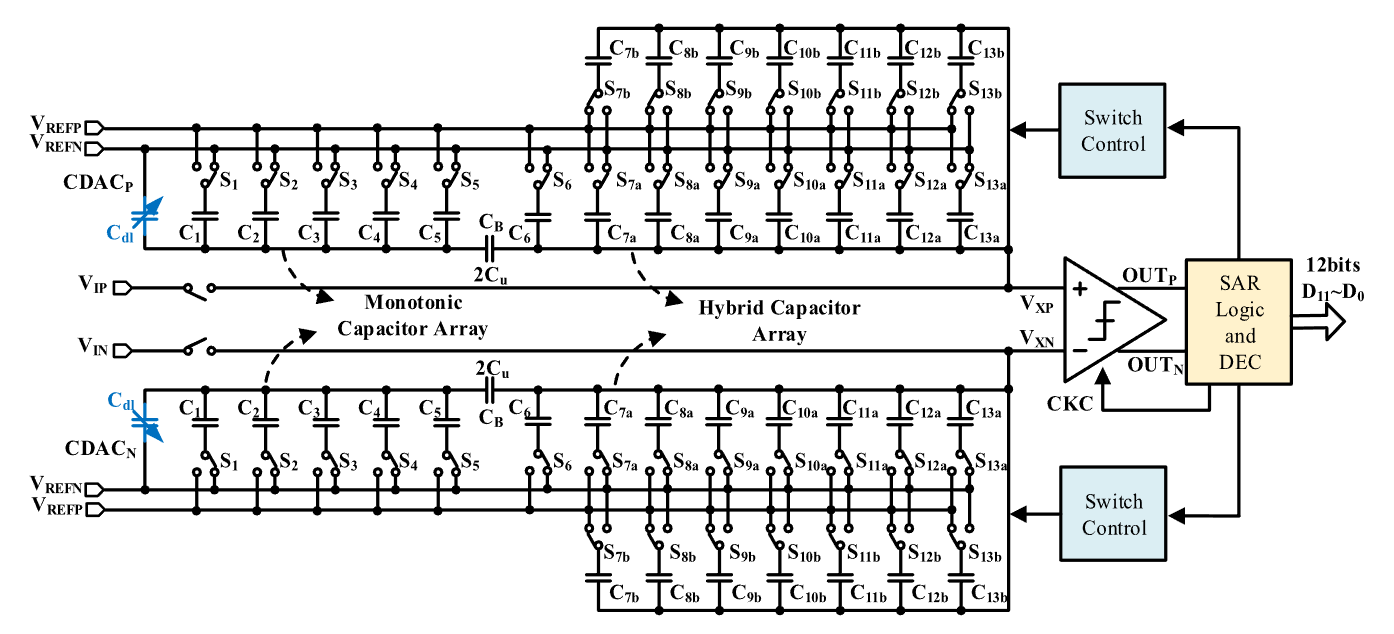
\includegraphics[width=1\textwidth]{Images/ADC-arch-paper.png}
    \caption{ADC architecture from the paper \textsuperscript{\cite{paper}}.}
    \label{fig:ADC-arch-paper}
\end{figure}

This ADC stands out for three architectural design choices that significantly enhance its performance:
\begin{itemize}
    \item Hybrid Capacitor Configuration;
    
    \item Split Capacitor Array;
    
    \item Asynchronous Logic.
\end{itemize}

We will delve into each of these design choices, providing a detailed explanation of their operation and the advantages they bring to the ADC.

In this report, the DEC error correction technique is not discussed, as it is not directly related to the ADC architecture. The DEC technique is a post-processing method that corrects errors in the digital output of the ADC, improving its overall performance. Thus, two pairs of capacitors were cut from the CDAC because they were used as redundant capacitors for the DEC technique. The architecture in study without the DEC technique is shown in Figure \ref{fig:ADC-sch-no-DEC}.

\begin{figure}[h]
    \centering
    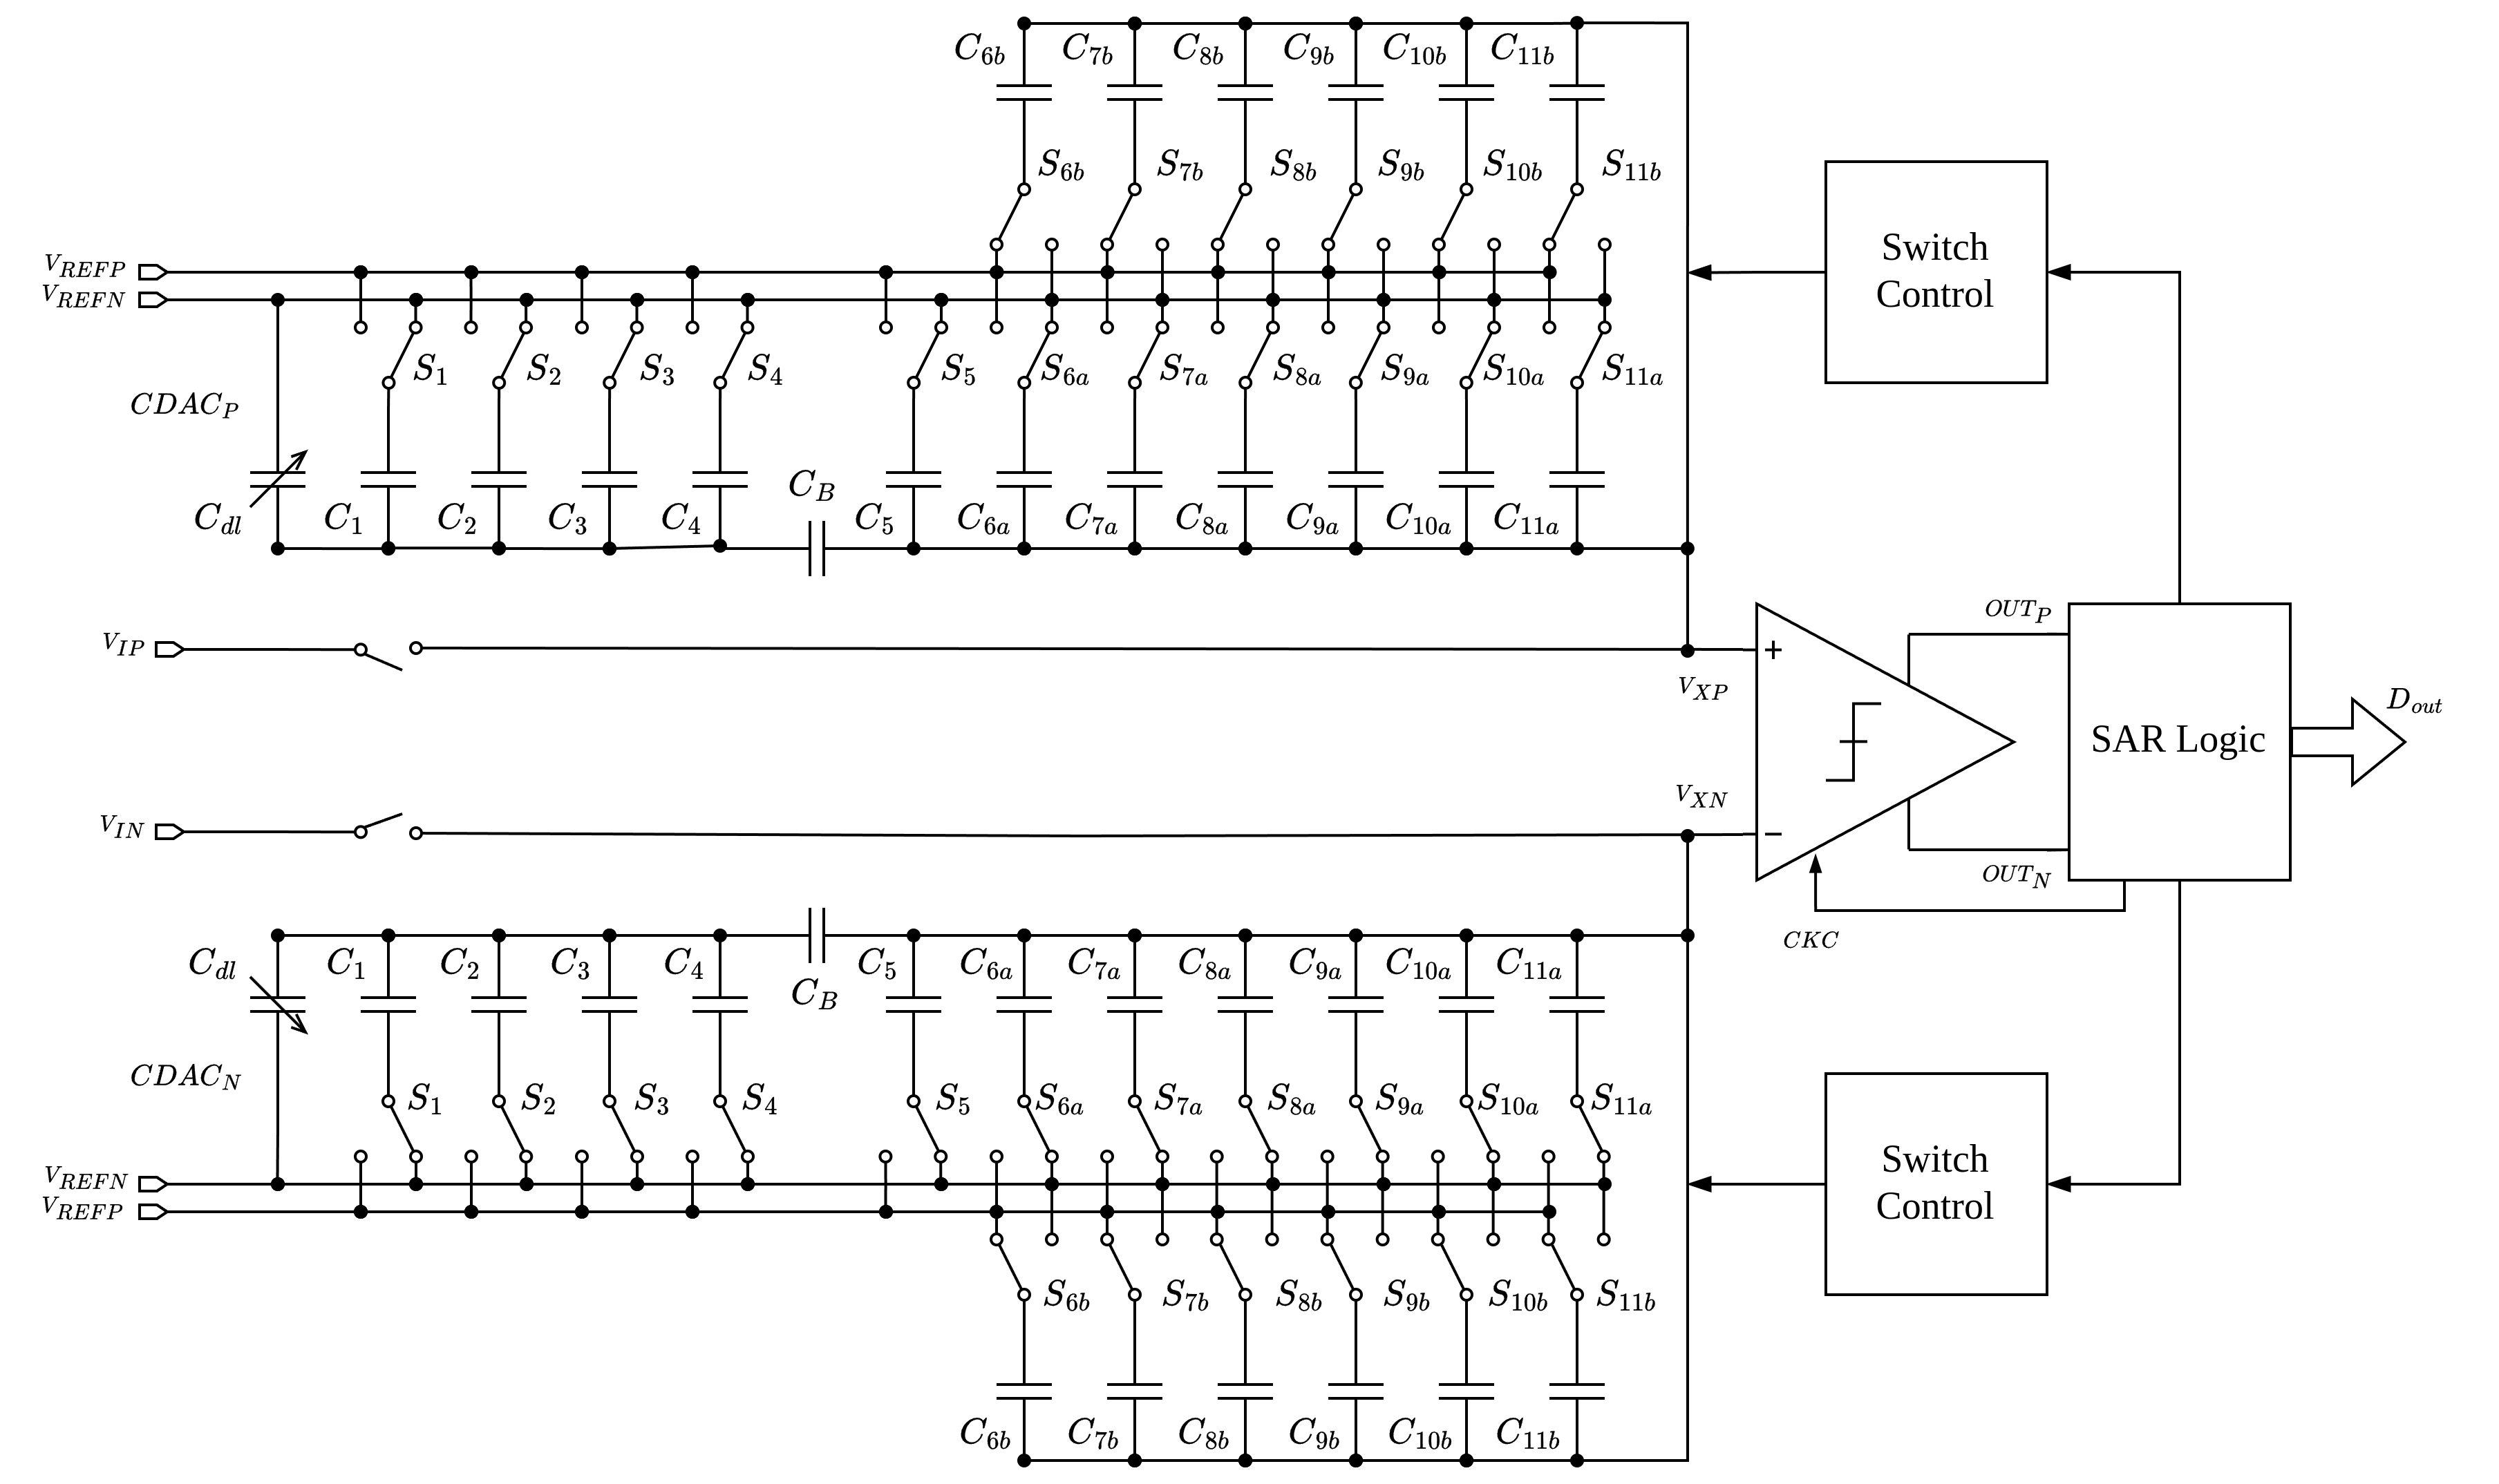
\includegraphics[width=0.8\textwidth]{Images/ADC-arch.png}
    \caption{ADC architecture without DEC redundant capacitors.}
    \label{fig:ADC-sch-no-DEC}
\end{figure}

\subsection{Top-Level Architecture}

Observing the top-level architecture of the ADC depicted in Figure \ref{fig:ADC-block-diagram}, we can identify the following key components:
\begin{itemize}
    \item Differential Input Sampling and Hold Stage: In this stage the bootstrapped switches are used to sample at $100 \si{\mega S \per \second}$ the differential input voltages ($V_{IP}$ and $V_{IN}$) onto the capacitors of the Capacitive-DAC 
    \item Capacitive-DAC;
    \item Dynamic comparator;
    \item Asynchronous SAR logic;
\end{itemize}

\begin{figure}[H]
    \centering
    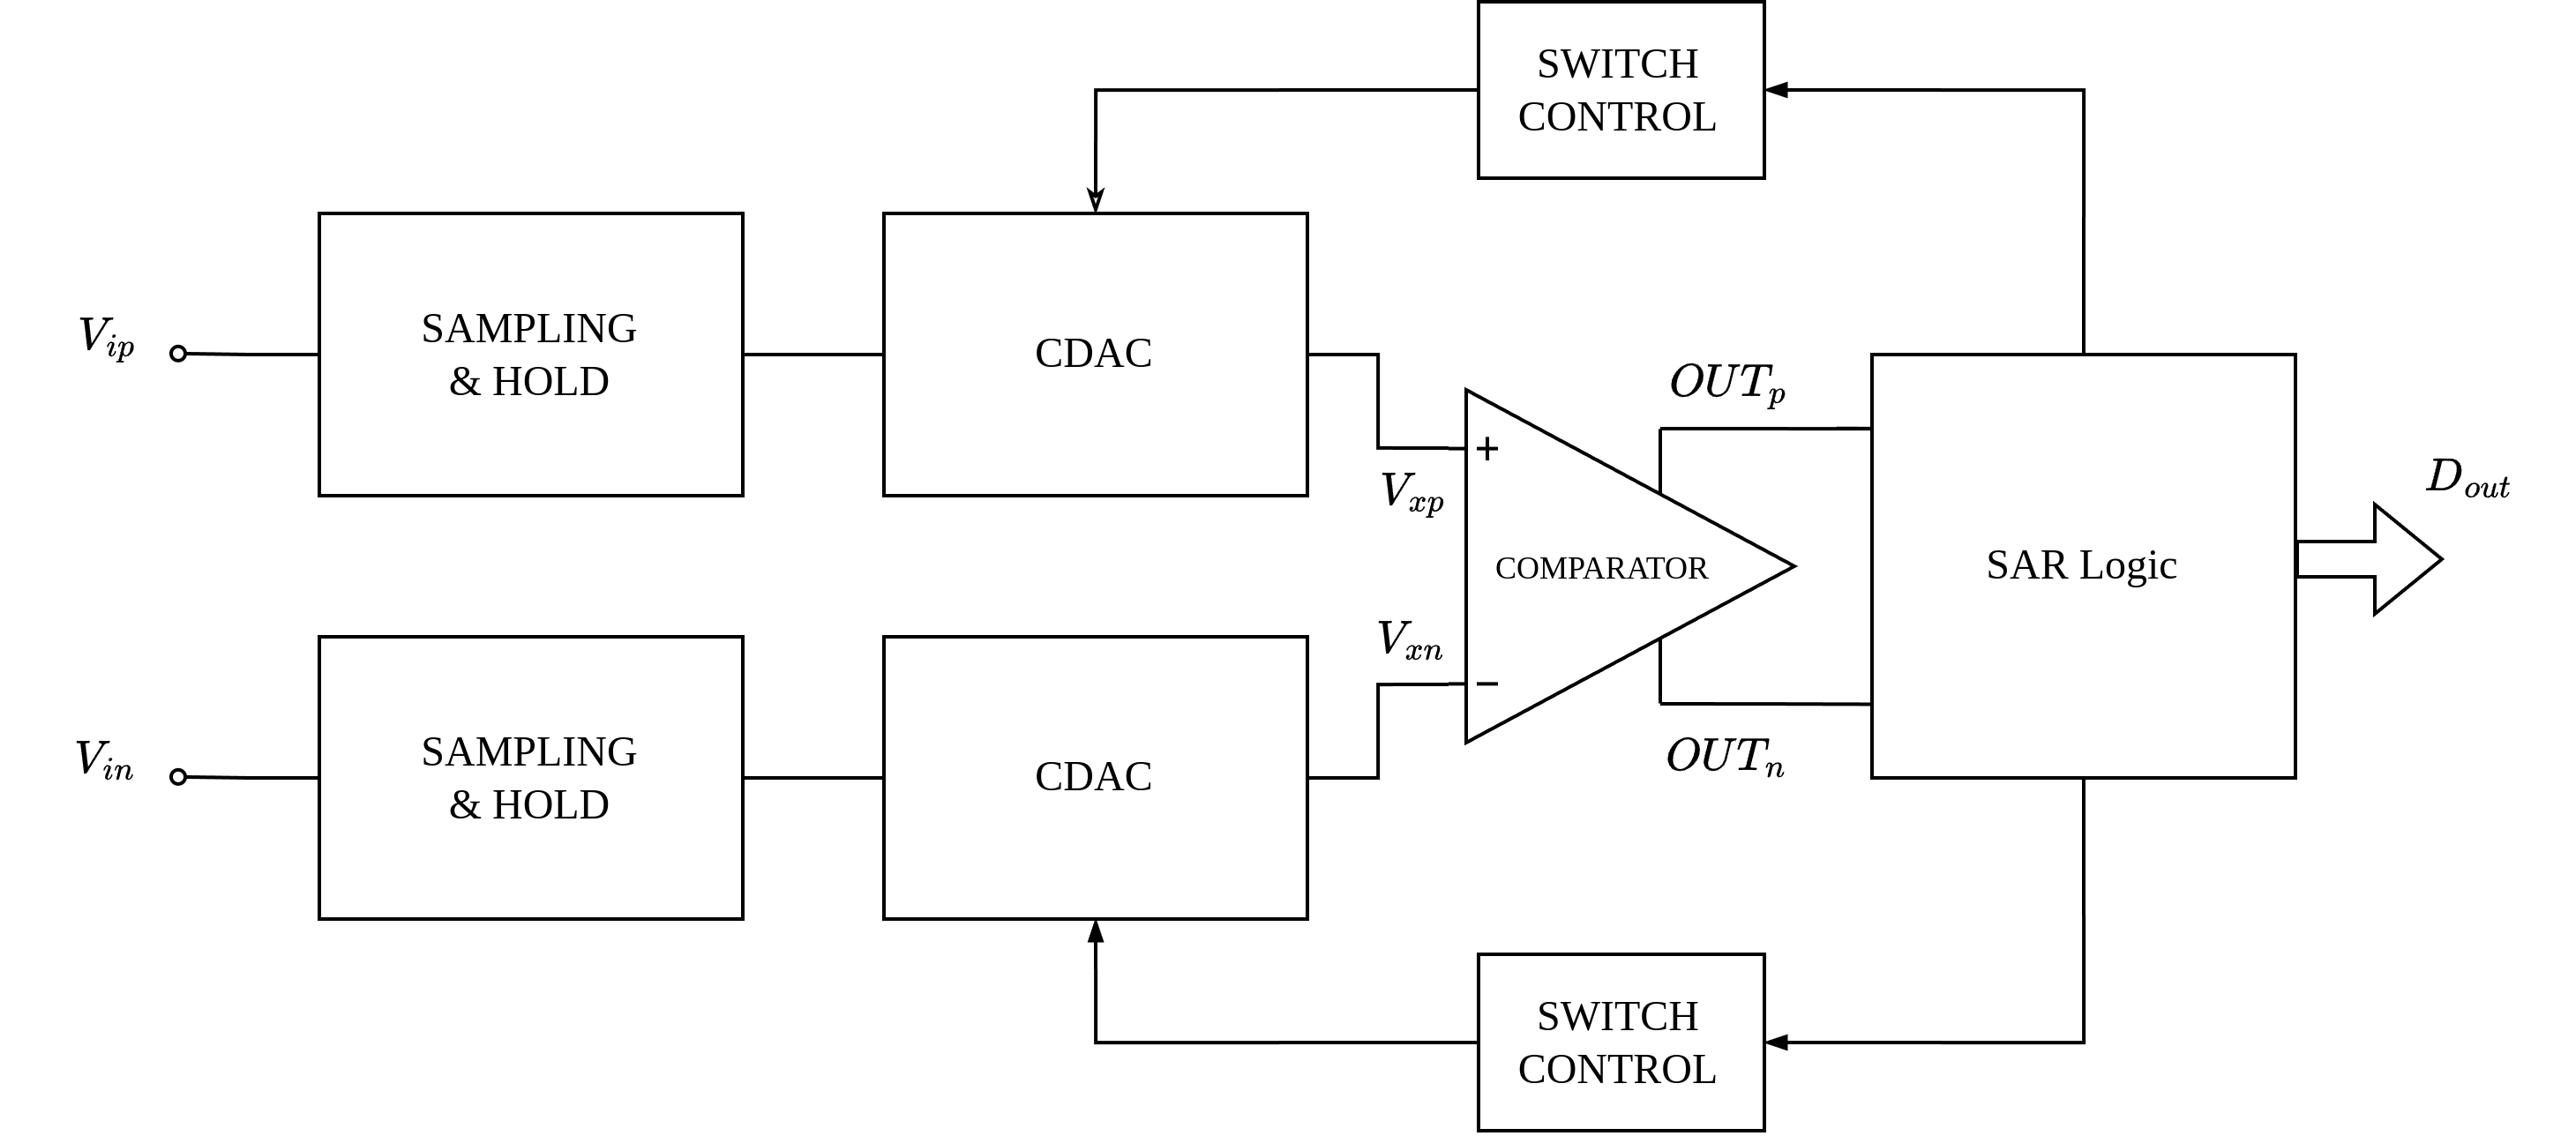
\includegraphics[width=0.7\textwidth]{Images/ADC-block-diagram.png}
    \caption{ADC simplified block diagram.}
    \label{fig:ADC-block-diagram}
\end{figure}

The ADC operates in a two-phase clocking scheme, where the first phase is dedicated to sampling the input voltages onto the capacitors of the Capacitive-DAC, while the second phase is used for the conversion process. The asynchronous SAR logic controls the DAC and performs a binary search, allowing for fast and efficient operation.

\subsection{Capacitive-DAC}
\label{sec:CDAC}
The Capacitive-DAC is a crucial component of the ADC, as it is responsible for converting the sampled input voltages into a digital representation. The CDAC consists of an array of capacitors that are switched to create a voltage divider network (used in binary search of the SAR logic block). The output voltage of the Capacitive-DAC is then compared to the reference voltage to determine the digital output of the ADC though the dynamic comparator. In this case since we have a fully differential ADC the reference voltage is the voltage of the symetric branch of the ADC, there is, the output voltage of the symetrical CDAC.

The C-DAC in study has a particular architecture that allows it to achieve high precision and low power consumption. 
For the sake of simplicity and because the circuit is symmetrical, we will only discuss the CDAC of one of branches, because they are equal. The CDAC implemented in each branch is shown in Figure \ref{fig:CDAC-sch}. 

\begin{figure}[h]
    \centering
    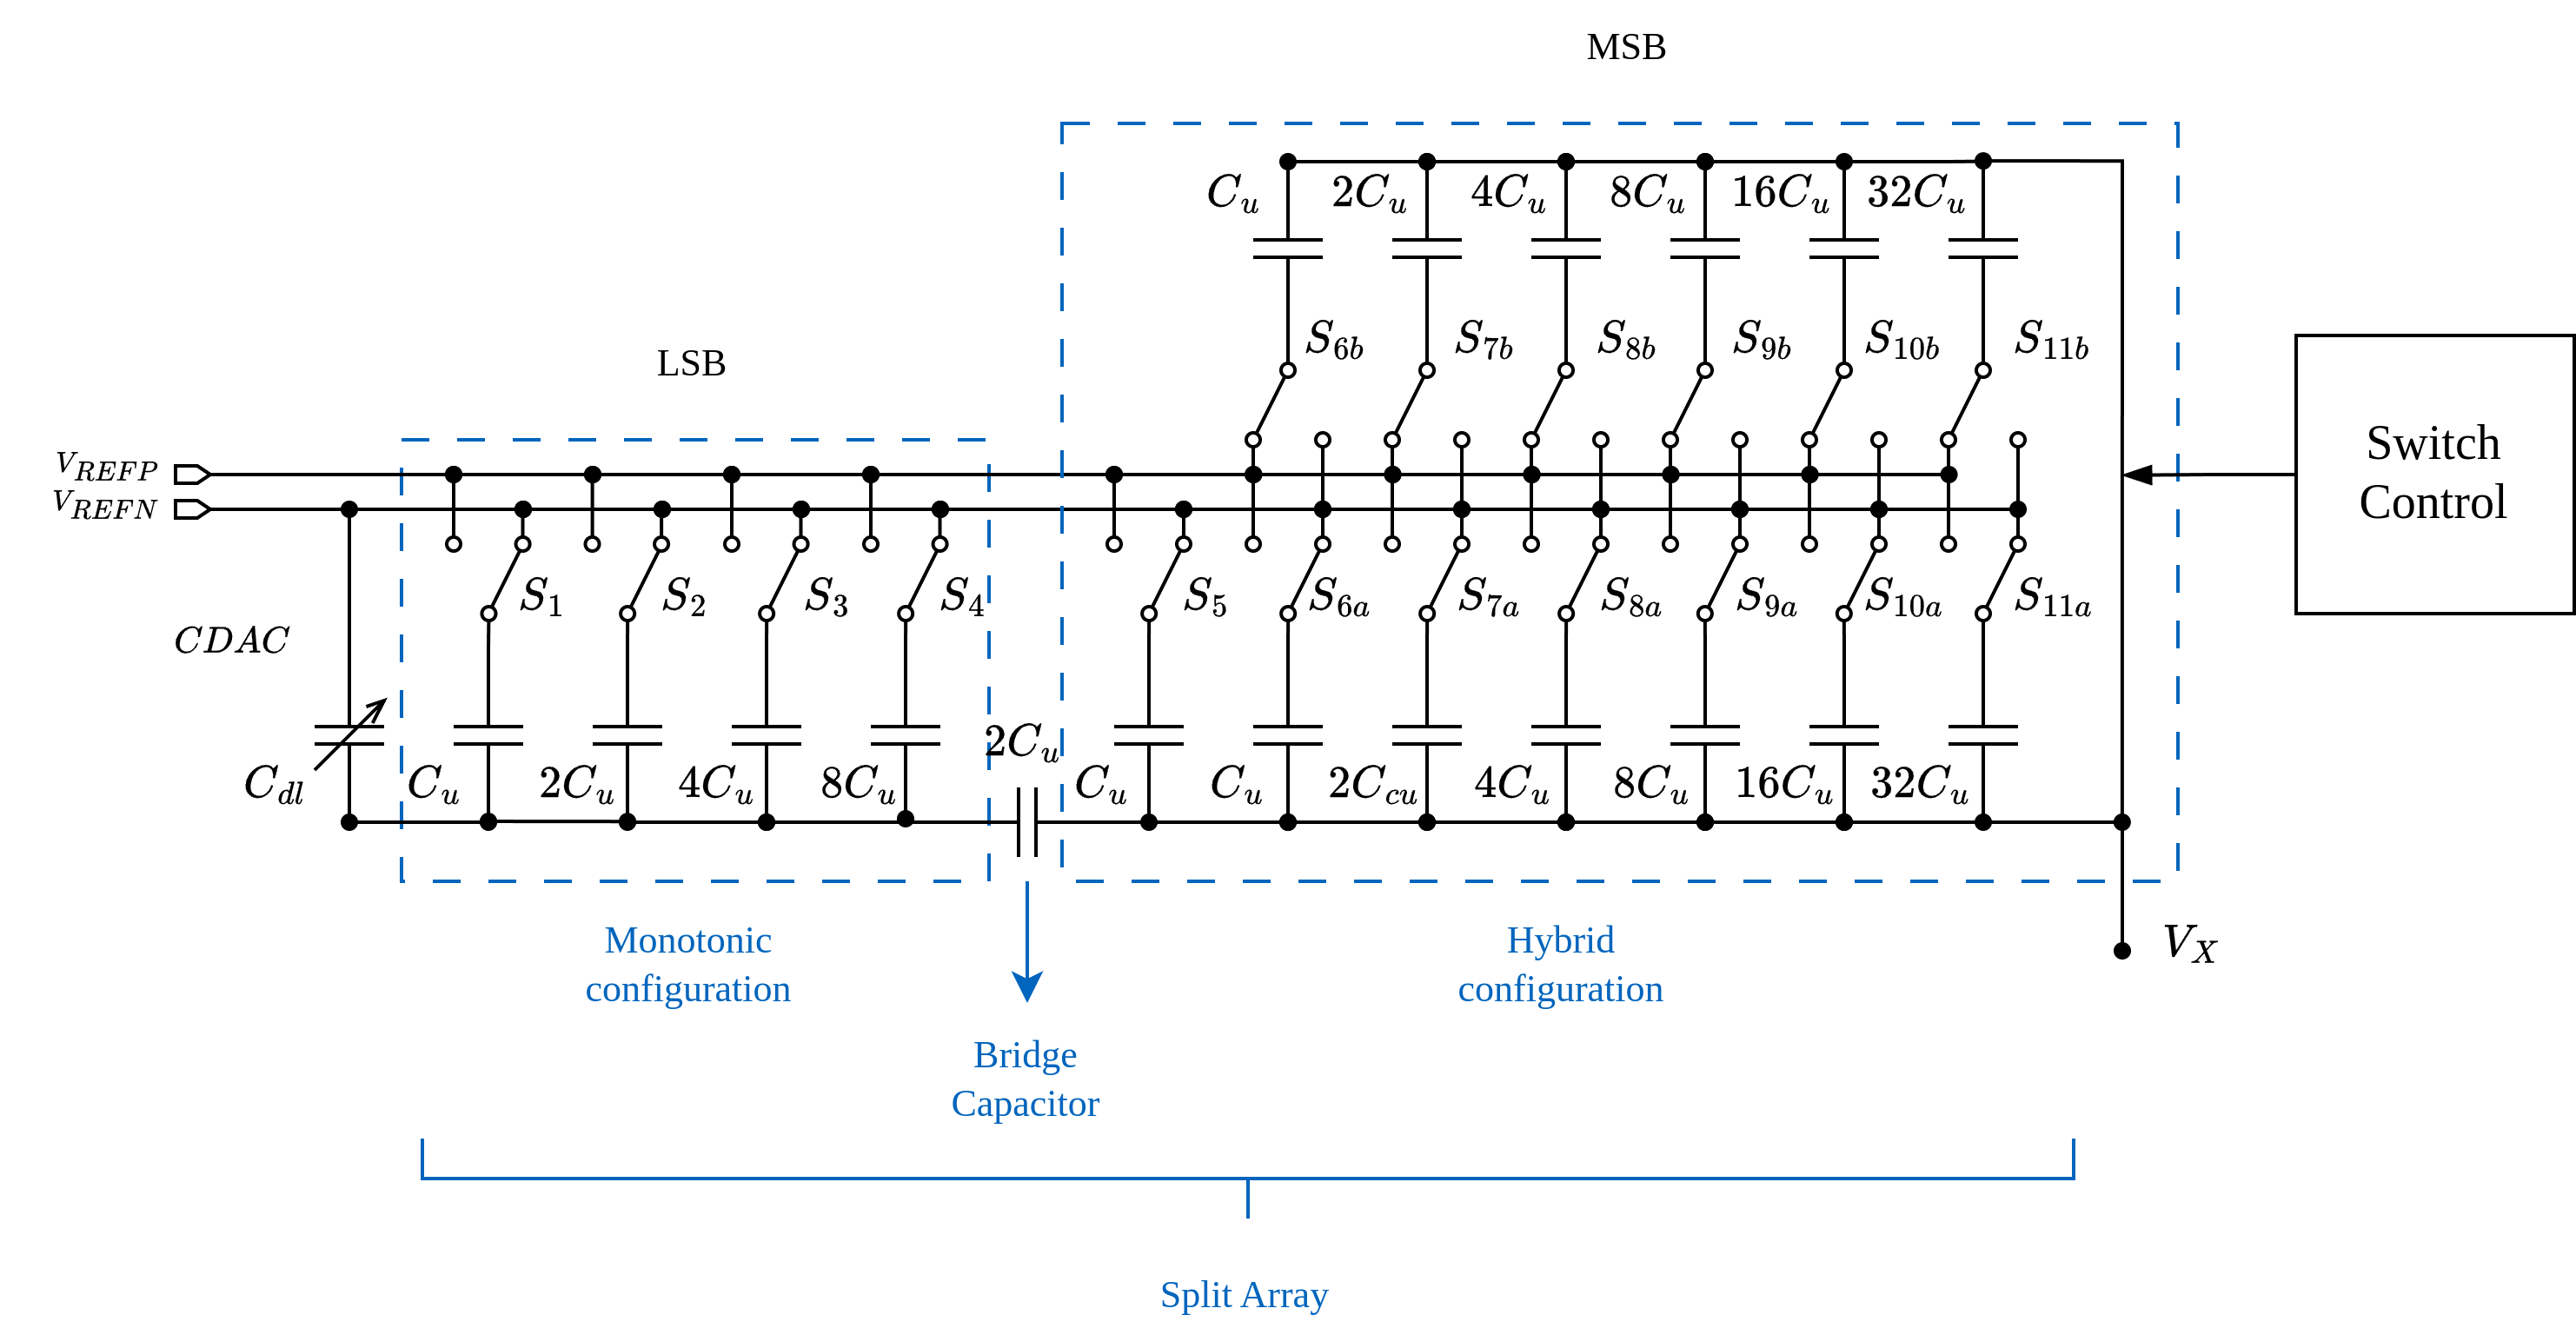
\includegraphics[width=1\textwidth]{Images/CDAC-sch.png}
    \caption{CDAC of one branch.}
    \label{fig:CDAC-sch}
\end{figure}

\subsubsection{Split Capacitor Array}

A split capacitor array is used to reduce the number of unit capacitors needed in comparison with a traditional binary-weighted capacitor array. It divides the capacitor array into two halves, the Most Significant Bit (MSB) and the Least Significant Bit (LSB) arrays. 

The reduction of unit capacitors has several advantages:

\textbf{Area occupation}
The split capacitor array requires fewer unit capacitors, which reduces the overall area of the ADC. This is particularly important in low-power applications where area is a critical constraint.

\textbf{Power consumption}
The reduced number of unit capacitors also leads to lower power consumption, as fewer capacitors need to be charged and discharged during the conversion process.

\textbf{Settling time}
The split capacitor array allows for faster settling times, as the MSB and LSB capacitors can be charged and discharged independently. This is particularly important in high-speed applications where fast conversion times are required.

In table \ref{tab:cap-numbers} we can see the number of capacitors used in the CDAC with the split capacitor array and a traditional binary-weighted capacitor array.

\begin{table}[h]
    \centering
    \caption{Comparison od CDAC architectures.}
    \begin{tabularx}{\textwidth}{>{\centering\arraybackslash}X >{\centering\arraybackslash}X}
        \toprule
        \textbf{CDAC Architecture} & \textbf{Number of Unit Capacitors} \\
        \midrule
        Split array & $2^{NLSB} -1 + 2^{NMSB} - 1 + C_B = 144C_u$\\
        \midrule
        Binary weighted array & $2^N = 2^{12} = 4095C_u$ \\
        \bottomrule
    \end{tabularx}
    \label{tab:cap-numbers}
\end{table}

\subsubsection{Hybrid Capacitor Configuration}  
The hybrid configuration is applied only to the MSB array, as it dominates DAC performance. The LSB array uses a traditional binary-weighted structure, the fact that it has smaller capacitors they have minimal impact in the common-mode voltage. Each MSB capacitor is split into two sub-capacitors ($C_{ia}$, $C_{ib}$). During sampling, $C_{ia}$ connects to $V_{\text{REFP}}$ (1.2 V) and $C_{ib}$ to $V_{\text{REFN}}$ (0 V). During conversion, only one sub-capacitor switches, while the other remains fixed. This design improves three key characteristics:  

\textbf{Common-Mode Voltage}  
Conventional SAR ADCs suffer from $V_{\text{cm}}$ fluctuations during capacitor switching, introducing noise and offset errors. By switching only one sub-capacitor, the hybrid configuration stabilizes $V_{\text{cm}}$ at 0.6 V (midpoint of $V_{\text{REFP}}$ and $V_{\text{REFN}}$). This reduces the kickback noise of the comparator and settling time, enabling a high ENOB.

\textbf{Energy Consumption}  
Traditional binary-weighted arrays require switching large capacitors, leading to high dynamic power. The hybrid configuration reduces energy by 50\%: only one sub-capacitor toggles per decision. In this way the energy consumed per conversion step is reduced.

\textbf{Linearity}  
Asymmetric charge injection in conventional designs degrades linearity (INL/DNL). The hybrid structure balances charge redistribution by switching one sub-capacitor while keeping the other fixed. A programmable dummy capacitor ($C_{dl}$) compensates the linearity error caused by the LSB array. This design choice enhances linearity.

\subsection{ADC Operation}

The process begins with the sampling of the input voltages ($V_{IP}$ and $V_{IN}$) onto the capacitors of the CDAC. The most significant bit of the CDACs are switched, and the dynamic comparator then compares the two output voltages of the CDACs ($V_{XN}$ and $V_{XP}$)and evaluate if the $V_{XP}$ is greater than $V_{XN}$ to determine the digital output of the ADC. 
The asynchronous SAR logic controls the conversion process, setting the next capacitors that generate the two new comparison voltages. The voltages change with the goal of reducing the difference between the two output voltages of the CDACs, this implementation is used to maintain differential balance since the switching is complementary for the two arrays.
The process continues until all 12 bits are converted, with the digital output being updated at each step. When the conversion is complete, the digital output, that is the binary value of difference between $V_{IP}$ and $V_{IN}$, becomes available, and the ADC is ready for the next conversion cycle. The flowchart in Figure \ref{fig:ADC-flowchart} illustrates the operation of the ADC.
\begin{figure}[H]
    \centering
    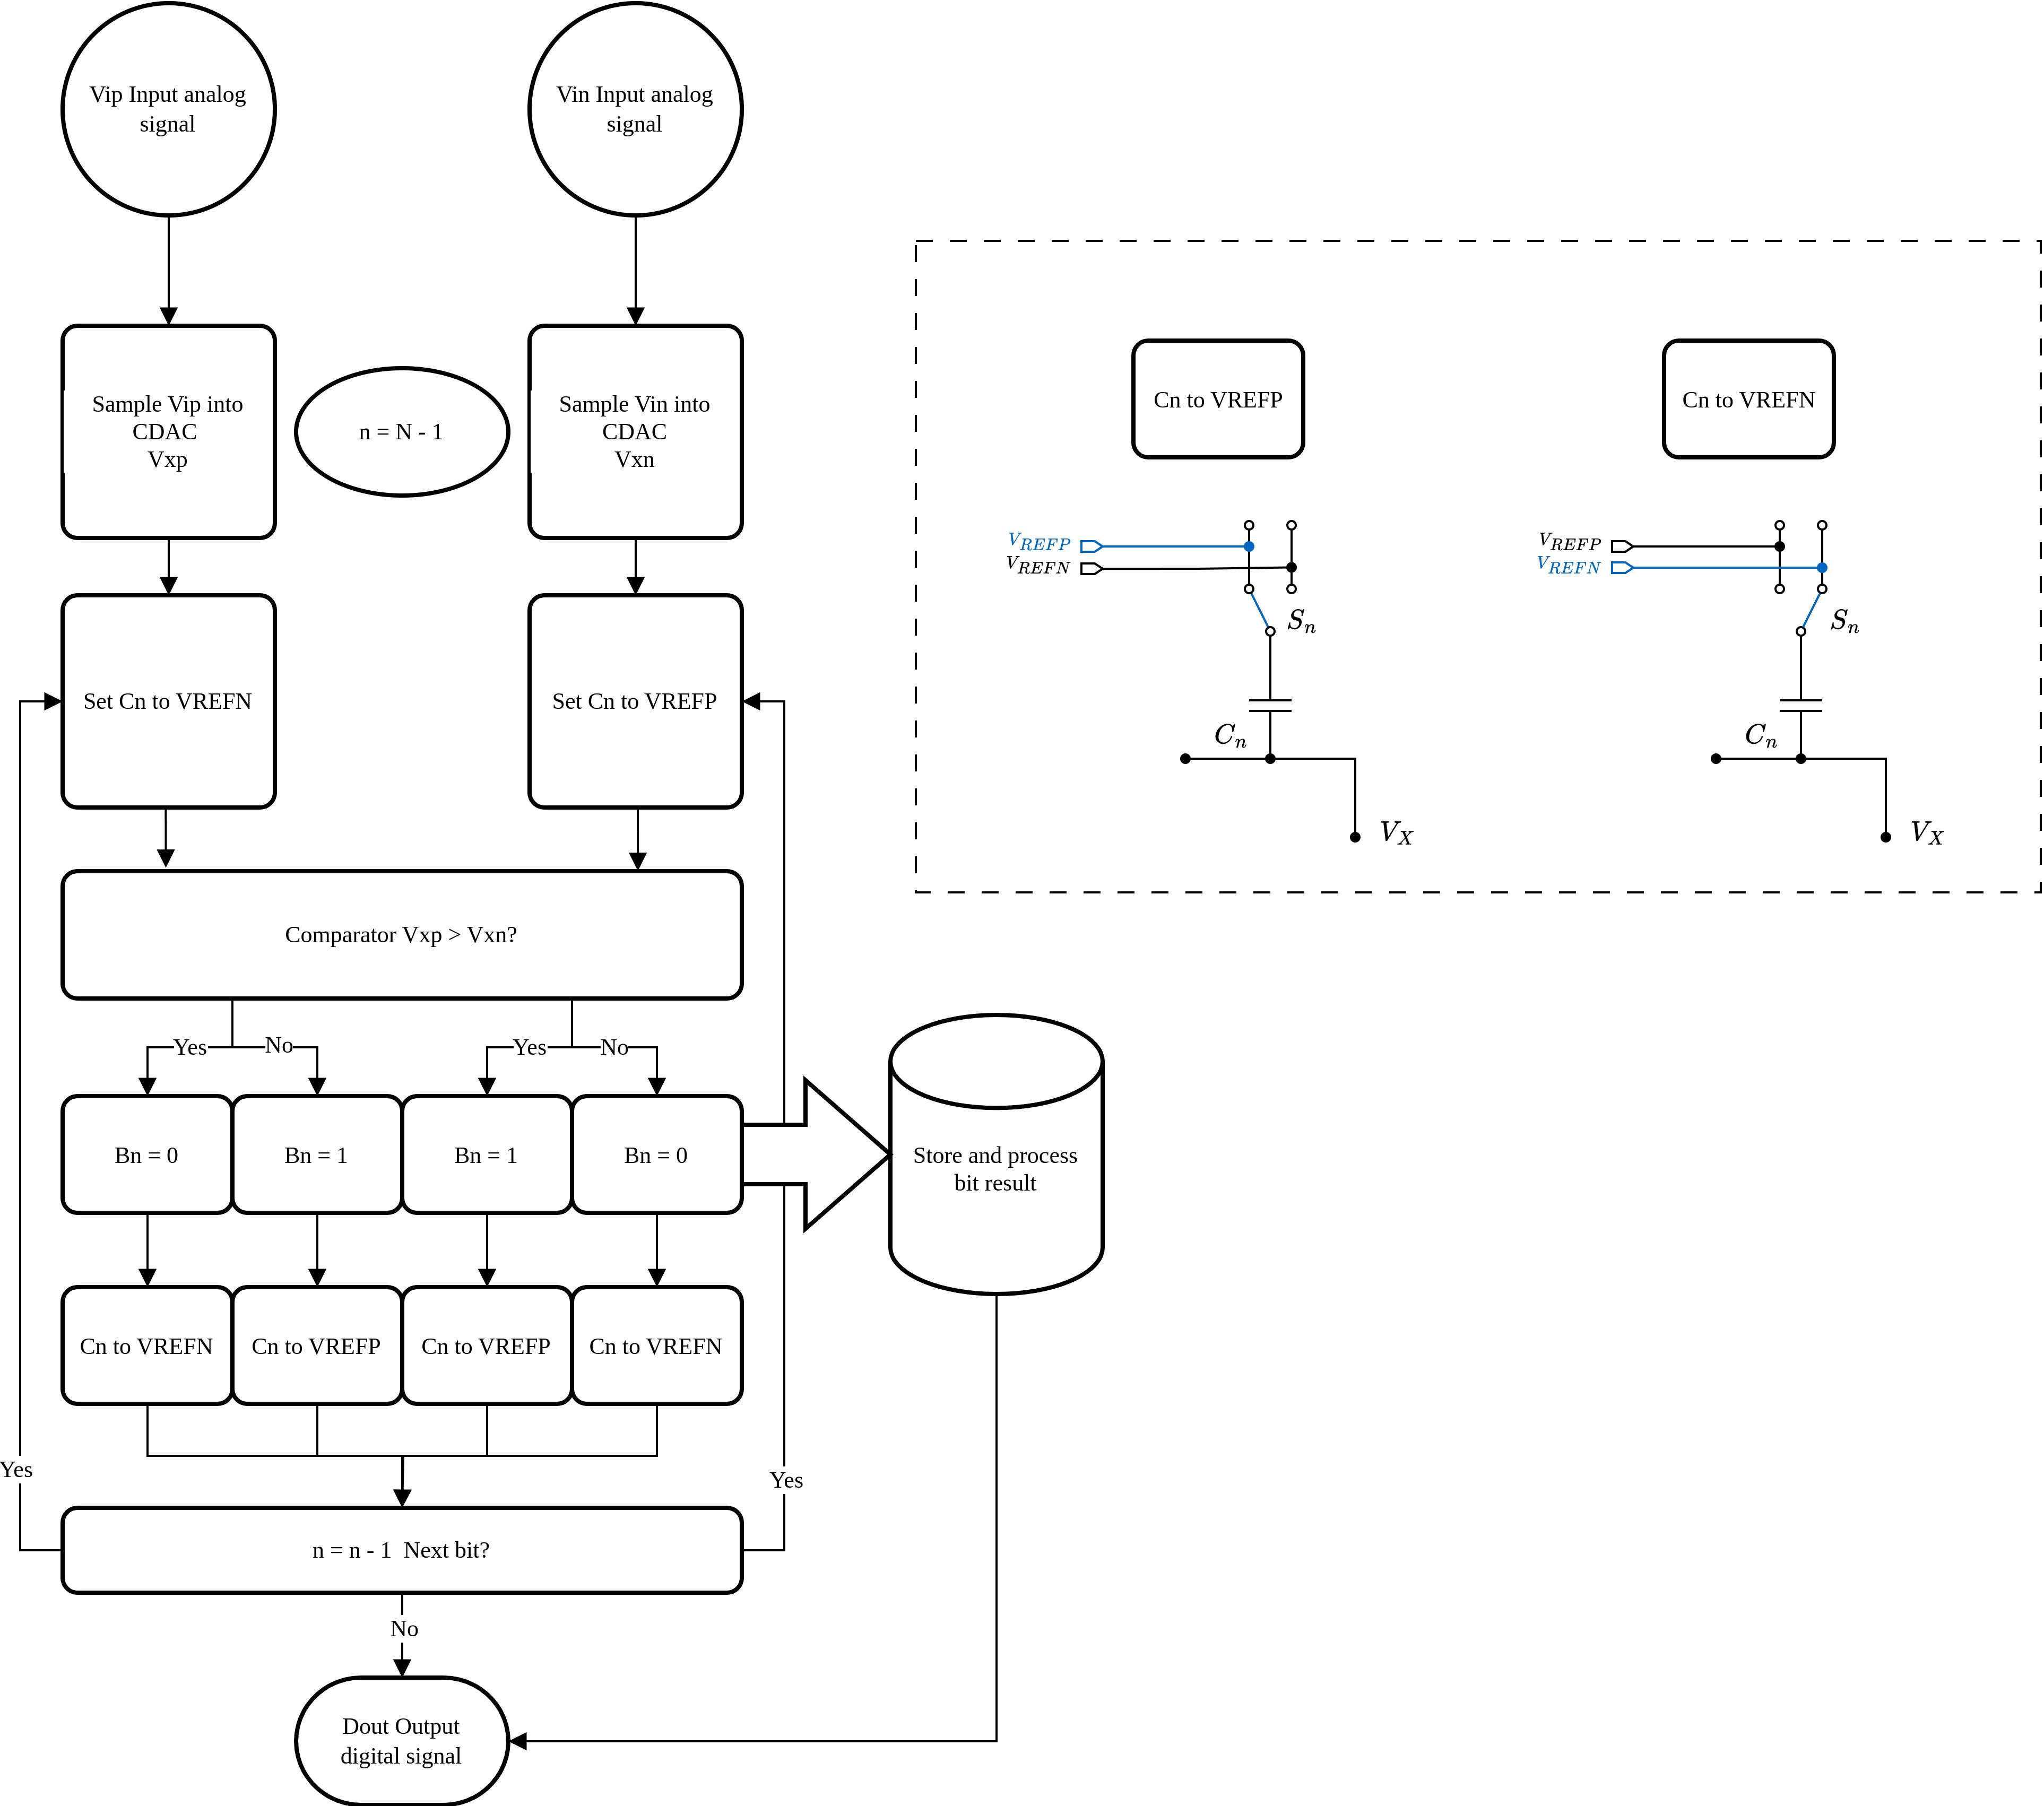
\includegraphics[width=0.9\textwidth]{Images/operation_ADC.png}
    \caption{ADC operation flowchart.}
    \label{fig:ADC-flowchart}
\end{figure}

% \textcolor{red}{Carefully read the paper to understand the operation of the ADC (Fig. 1). If necessary, obtain and read papers cited by this paper. Explain why the authors decided to use a hybrid capacitor configuration and why they use the split capacitor array.}